

\tikzset{every picture/.style={line width=0.75pt}} %set default line width to 0.75pt        

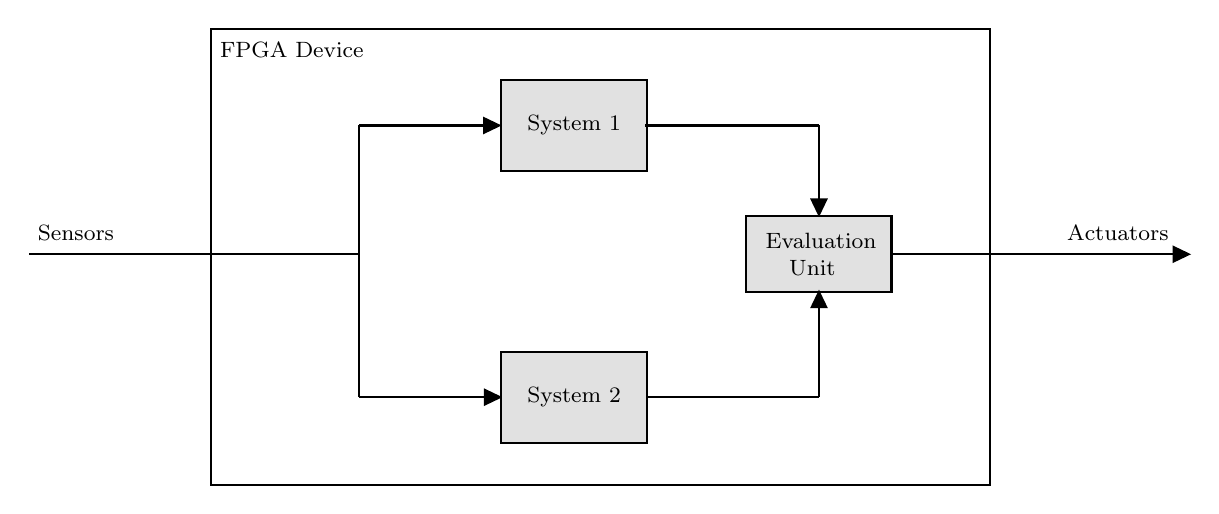
\begin{tikzpicture}[x=0.75pt,y=0.75pt,yscale=-1,xscale=1]
%uncomment if require: \path (0,300); %set diagram left start at 0, and has height of 300

%Straight Lines [id:da5881950910157023] 
\draw    (286.51,183) -- (220.3,183) ;

\draw [shift={(289.51,183)}, rotate = 180] [fill={rgb, 255:red, 0; green, 0; blue, 0 }  ][line width=0.08]  [draw opacity=0] (8.93,-4.29) -- (0,0) -- (8.93,4.29) -- cycle    ;
%Straight Lines [id:da25338917902177904] 
\draw    (220.3,52.09) -- (220.3,183) ;


%Shape: Rectangle [id:dp3450500434713657] 
\draw  [fill={rgb, 255:red, 225; green, 225; blue, 225 }  ,fill opacity=1 ] (289.05,161.14) -- (359.05,161.14) -- (359.05,204.86) -- (289.05,204.86) -- cycle ;
%Shape: Rectangle [id:dp14922514498310435] 
\draw  [fill={rgb, 255:red, 225; green, 225; blue, 225 }  ,fill opacity=1 ] (289.05,30.23) -- (359.05,30.23) -- (359.05,73.95) -- (289.05,73.95) -- cycle ;
%Straight Lines [id:da0868762150769582] 
\draw    (286.12,52.09) -- (220.3,52.09) ;

\draw [shift={(289.12,52.09)}, rotate = 180] [fill={rgb, 255:red, 0; green, 0; blue, 0 }  ][line width=0.08]  [draw opacity=0] (8.93,-4.29) -- (0,0) -- (8.93,4.29) -- cycle    ;
%Straight Lines [id:da9680613737529542] 
\draw    (220.3,114.14) -- (61.3,114.14) ;


%Shape: Rectangle [id:dp2265192536845475] 
\draw  [fill={rgb, 255:red, 225; green, 225; blue, 225 }  ,fill opacity=1 ] (407.1,95.86) -- (476.99,95.86) -- (476.99,132.42) -- (407.1,132.42) -- cycle ;
%Straight Lines [id:da668687133025897] 
\draw    (442.05,134.2) -- (442.05,183) ;

\draw [shift={(442.05,131.2)}, rotate = 90] [fill={rgb, 255:red, 0; green, 0; blue, 0 }  ][line width=0.08]  [draw opacity=0] (8.93,-4.29) -- (0,0) -- (8.93,4.29) -- cycle    ;
%Straight Lines [id:da3164126413280457] 
\draw    (442.05,93.2) -- (442.05,52.09) ;

\draw [shift={(442.05,96.2)}, rotate = 270] [fill={rgb, 255:red, 0; green, 0; blue, 0 }  ][line width=0.08]  [draw opacity=0] (8.93,-4.29) -- (0,0) -- (8.93,4.29) -- cycle    ;
%Straight Lines [id:da2018473186011438] 
\draw    (442.05,183) -- (359.3,183) ;


%Straight Lines [id:da8685031016449603] 
\draw    (442.05,52.09) -- (358.3,52.09) ;


%Straight Lines [id:da7841339318502909] 
\draw    (618.3,114.14) -- (477.3,114.14) ;

\draw [shift={(621.3,114.14)}, rotate = 180] [fill={rgb, 255:red, 0; green, 0; blue, 0 }  ][line width=0.08]  [draw opacity=0] (8.93,-4.29) -- (0,0) -- (8.93,4.29) -- cycle    ;
%Shape: Rectangle [id:dp3914738316121473] 
\draw   (149.3,5.47) -- (524.3,5.47) -- (524.3,225.2) -- (149.3,225.2) -- cycle ;

% Text Node
\draw (324.05,52.09) node  [font=\footnotesize] [align=left] {System 1};
% Text Node
\draw (324.05,183) node  [font=\footnotesize] [align=left] {System 2};
% Text Node
\draw (443.05,114.14) node  [font=\footnotesize] [align=left] {Evaluation\\ \ \ \ Unit};
% Text Node
\draw (586.05,103.64) node  [font=\footnotesize] [align=left] {Actuators};
% Text Node
\draw (84.05,103.64) node  [font=\footnotesize] [align=left] {Sensors};
% Text Node
\draw (188.05,15.59) node  [font=\footnotesize] [align=left] {FPGA Device};


\end{tikzpicture}
